\documentclass[11pt, a4paper, twoside]{article}   	% use "amsart" instead of "article" for AMSLaTeX format

\usepackage{geometry}                		% See geometry.pdf to learn the layout options. There are lots.
\usepackage{pdfpages}
\usepackage{caption}
\usepackage{minted}
\usepackage[german]{babel}			% this end the next are needed for german umlaute
\usepackage[utf8]{inputenc}
\usepackage{color}
\usepackage{graphicx}
\usepackage{titlesec}
\usepackage{fancyhdr}
\usepackage{lastpage}
\usepackage{hyperref}
\usepackage[autostyle=false, style=english]{csquotes}
\usepackage{mathtools}
\usepackage{tabularx}
% http://www.artofproblemsolving.com/wiki/index.php/LaTeX:Symbols#Operators
% =============================================
% Layout & Colors
% =============================================
\geometry{
   a4paper,
   total={210mm,297mm},
   left=20mm,
   right=20mm,
   top=20mm,
   bottom=30mm
 }	

\definecolor{myred}{rgb}{0.8,0,0}
\definecolor{mygreen}{rgb}{0,0.6,0}
\definecolor{mygray}{rgb}{0.5,0.5,0.5}
\definecolor{mymauve}{rgb}{0.58,0,0.82}

\setcounter{secnumdepth}{4}


% the default java directory structure and the main packages
\newcommand{\srcDir}{../src/}
\newcommand{\imageDir}{./images/}
% =============================================
% Code Settings
% =============================================
\newenvironment{code}{\captionsetup{type=listing}}{}
\newmintedfile[mSourceFile]{matlab}{
	linenos=true, 
	frame=single, 
	breaklines=true, 
	tabsize=2,
	numbersep=5pt,
	xleftmargin=10pt,
	baselinestretch=1,
	fontsize=\footnotesize
}
\newmintinline[mInlineSource]{matlab}{}
\newminted[mSource]{matlab}{
	breaklines=true, 
	tabsize=2,
	autogobble=true,
	breakautoindent=false
}
% =============================================
% Page Style, Footers & Headers, Title
% =============================================
\title{Übung 1}
\author{Thomas Herzog}

\lhead{Übung 1}
\chead{}
\rhead{
\includegraphics[scale=0.10]{FHO_Logo_Students.jpg}}

\lfoot{S1610454013}
\cfoot{}
\rfoot{ \thepage / \pageref{LastPage} }
\renewcommand{\footrulewidth}{0.4pt}
% =============================================
% D O C U M E N T     C O N T E N T
% =============================================
% =============================================
% 2016.10.13: 1 
% 2016.10.14: 2
% =============================================

\pagestyle{fancy}
\begin{document}
\setlength{\headheight}{15mm}
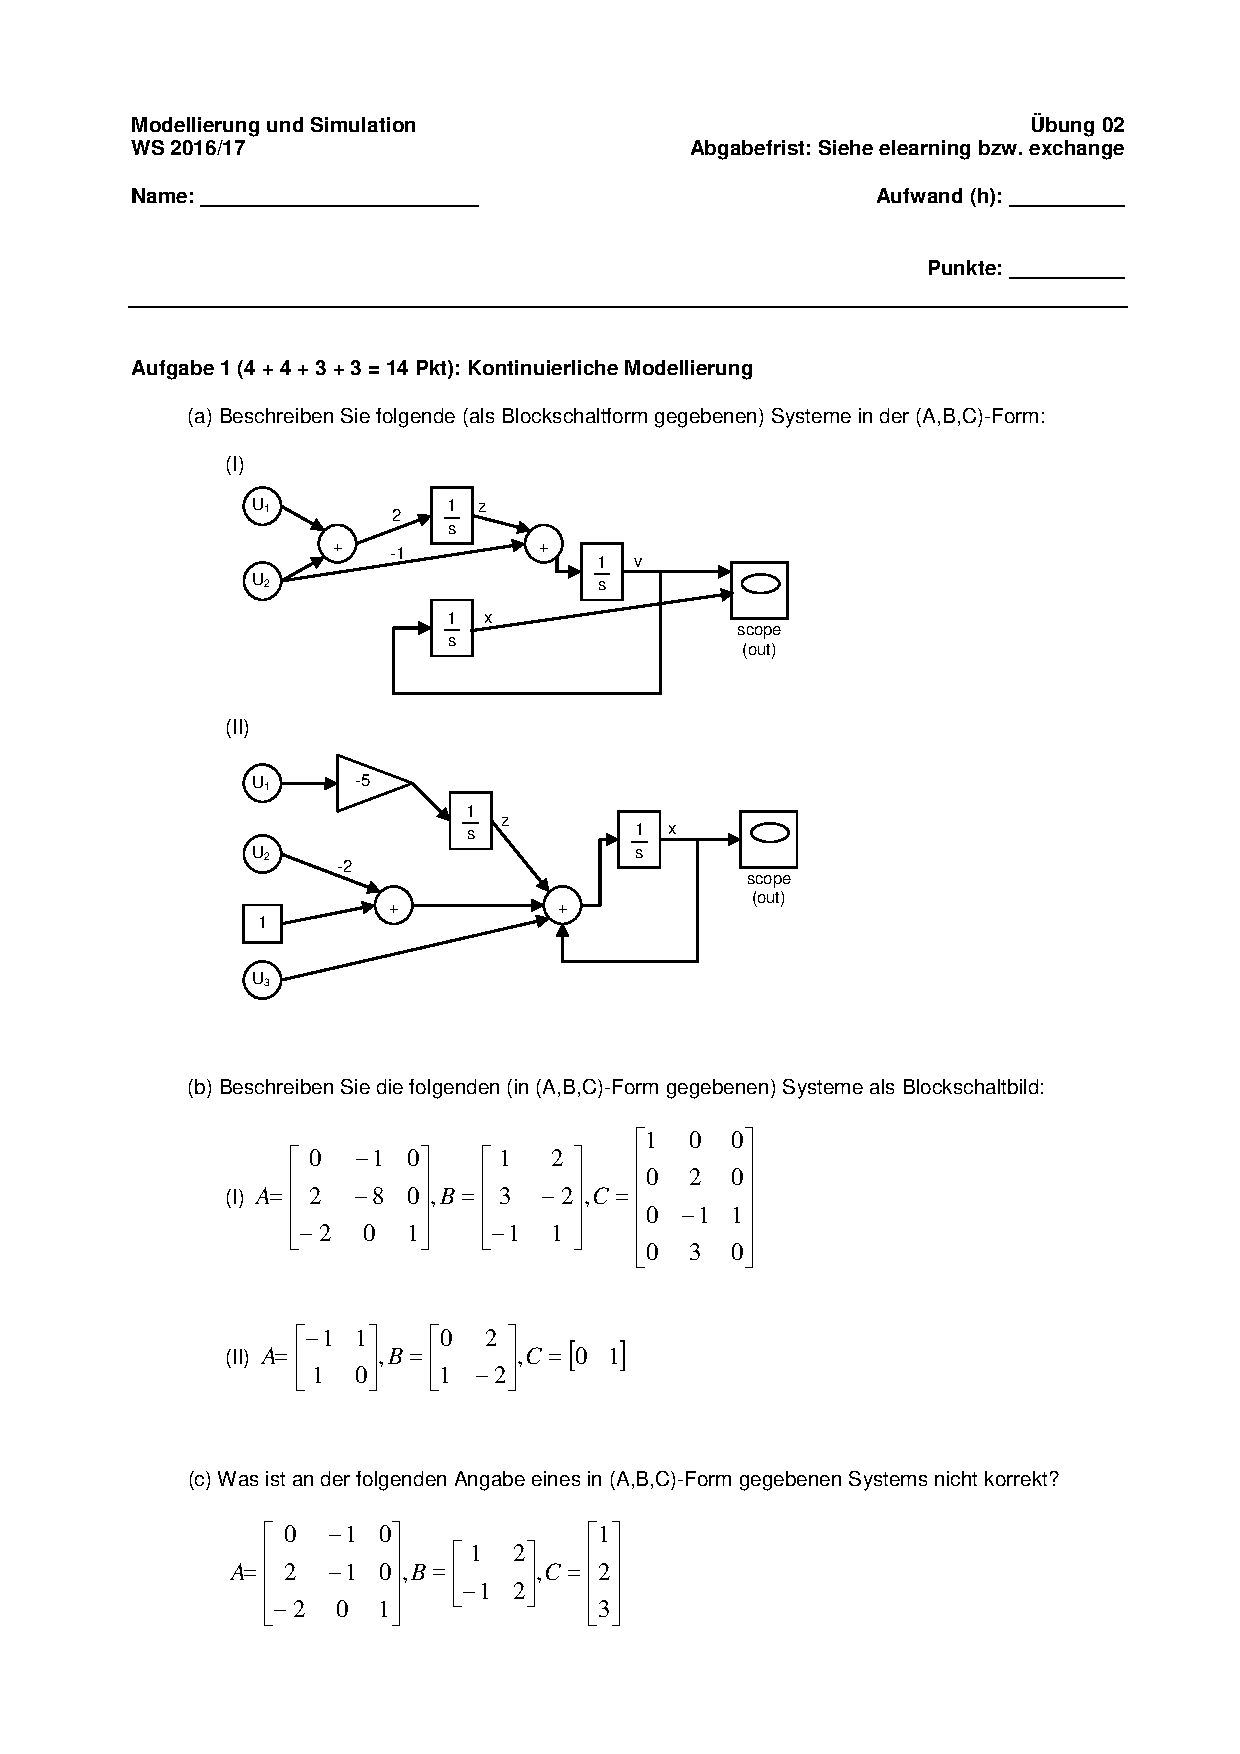
\includepdf[pages={1,2}]{Uebungszettel02.pdf}

% Section gramar and basics 
\section{Kontinuierliche Modellierung}
\label{sec:continous-modeling}
Dieser Abschnitt beschäftigt sich mit der Aufgabenstellung 1 der zweiten Übung. 

\subsection{Erstes Blockdiagramm}
Dieser Abschnitt beschäftigt ich mit dem Aufstellen der Gleichungen in A, B, C Normalform, die aus den gegebenen Blockdiagramm abgeleitet wurden.
\newline
\newline
$U= \begin{bmatrix}
	u_1 \\[0.3em]
	u_2 \\[0.3em]
\end{bmatrix}
,
X = \begin{bmatrix}
	z \\[0.3em]
	v \\[0.3em]
	x \\[0.3em]
\end{bmatrix}
,
Y=\begin{bmatrix}
	y_1 \\[0.3em]
	y_2 \\[0.3em]
	y_3 \\[0.3em]
\end{bmatrix}
\newline
\newline
\newline
z'= 0*z + 0*v + 0*x + 2*u_1 + 2*u_2 \hspace{2mm} \equiv \hspace{2mm} 2*u_1 + 2*u_2
\newline
v'= 1*z + 0*v + 0*x + 0*u_1 - 1*u_2 \hspace{2mm} \equiv \hspace{2mm} z - u_2
\newline
x'= 0*z + 1*v + 0*x + 0*u_1 + 0*u_2 \hspace{2mm} \equiv \hspace{2mm} v 
\newline
\newline
y_1 = 0*z + 0*v + 0* x \hspace{30mm} \equiv \hspace{2mm} 0
\newline
y_2 = 0*z + 1*v + 0* x \hspace{30mm} \equiv \hspace{2mm} v
\newline
y_3 = 0*z + 0*v + 1* x \hspace{30mm} \equiv \hspace{2mm} x
\newline
\newline
\newline
X'=A*X + B * U
\newline
\newline
X'= \begin{bmatrix}
	0 & 0 & 0 \\[0.3em]
	1 & 0 & 0 \\[0.3em]
	0 & 1 & 0 \\[0.3em]
\end{bmatrix}
* 
\begin{bmatrix}
	z \\[0.3em]
	v \\[0.3em]
	x \\[0.3em]
\end{bmatrix}
+
\begin{bmatrix}
	2 & 2\\[0.3em]
	0 & -1 \\[0.3em]
	0 & 0 \\[0.3em]
\end{bmatrix}
*
\begin{bmatrix}
	u_1 \\[0.3em]
	u_2 \\[0.3em]
\end{bmatrix}
\newline
\newline
\newline
\newline
Y=C*X
\newline
\newline
Y=
\begin{bmatrix}
	0 & 0 & 0 \\[0.3em]
	0 & 1 & 0 \\[0.3em]
	0 & 0 & 1 \\[0.3em]
\end{bmatrix}
*
\begin{bmatrix}
	z \\[0.3em]
	v \\[0.3em]
	x \\[0.3em]
\end{bmatrix}
$
\newpage

\subsection{Zweites Blockdiagramm}
Dieser Abschnitt beschäftigt ich mit dem Aufstellen der Gleichungen in A, B, C Normalform, die aus den gegebenen Blockdiagramm abgeleitet wurden.
\newline
\newline
$U= \begin{bmatrix}
	u_1 \\[0.3em]
	u_2 \\[0.3em]
	u_3 \\[0.3em]
\end{bmatrix}
,
X = \begin{bmatrix}
	z \\[0.3em]
	x \\[0.3em]
\end{bmatrix}
,
Y = \begin{bmatrix}
	y1 \\[0.3em]
	y2 \\[0.3em]
\end{bmatrix}
\newline
\newline
\newline
z'= 0*z + 0*x + 0*u_1 - 5*u_2 + 0*u_3\hspace{15mm} \equiv \hspace{2mm} - 5*u_2
\newline
x'= 1*z + 1*x + 0*u_1 + (-2*u_2 + 1) + 1*u_3 \hspace{2mm} \equiv \hspace{2mm} z + x + (-2*u_2 + 1) + u_3
\newline
\newline
y_1 = 0*z + 0* x \hspace{57mm} \equiv \hspace{2mm} 0
\newline
y_2 = 0*z + 1* x \hspace{57mm} \equiv \hspace{2mm} x
\newline
\newline
\newline
X'=A*X + B * U
\newline
\newline
X'= \begin{bmatrix}
	0 & 0 \\[0.3em]
	1 & 1 \\[0.3em]
\end{bmatrix}
* 
\begin{bmatrix}
	z \\[0.3em]
	x \\[0.3em]
\end{bmatrix}
+
\begin{bmatrix}
	0 & -5 & 0 \\[0.3em]
	0 & (-2*u_2 + 1) & 1 \\[0.3em]
\end{bmatrix}
*
\begin{bmatrix}
	u_1 \\[0.3em]
	u_2 \\[0.3em]
	u_3 \\[0.3em]
\end{bmatrix}
\newline
\newline
\newline
\newline
Y=C*X
\newline
\newline
Y =
C = \begin{bmatrix}
	0 & 0 \\[0.3em]
	0 & 1 \\[0.3em]
\end{bmatrix}
*
\begin{bmatrix}
	z \\[0.3em]
	x \\[0.3em]
\end{bmatrix}
$
\newpage

\subsection{Erstes System als Blockschaltbild}
$
U= \begin{bmatrix}
	u_1 \\[0.3em]
	u_2 \\[0.3em]
\end{bmatrix}
,
X = \begin{bmatrix}
	x \\[0.3em]
	v \\[0.3em]
	z \\[0.3em]
\end{bmatrix}
$
\begin{figure}[h]
\centering
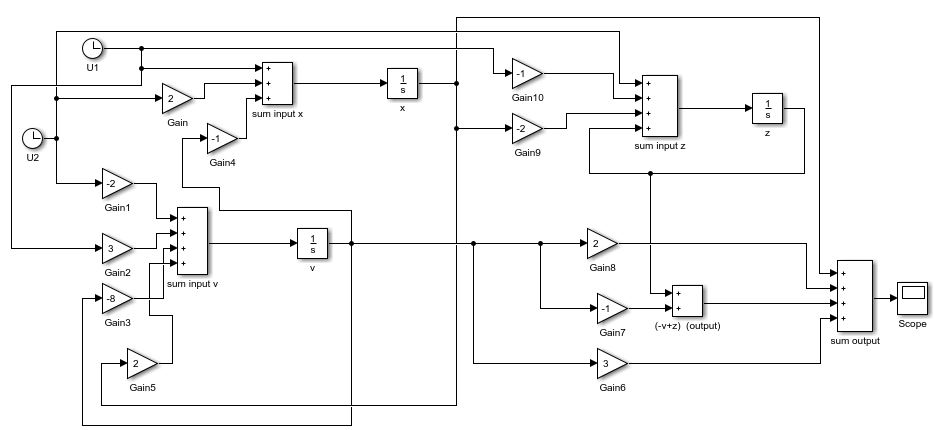
\includegraphics[scale=0.70,angle=90]{\imageDir/aufgabe_b1.JPG}
\caption{Blockschaltbild zum System aus Aufgabe b1}
\label{fig:exercise-b1}
\end{figure}
\newpage

\subsection{Zweites System als Blockschaltbild}
$
U= \begin{bmatrix}
	u_1 \\[0.3em]
	u_2 \\[0.3em]
\end{bmatrix}
,
X = \begin{bmatrix}
	x \\[0.3em]
	v \\[0.3em]
\end{bmatrix}
\newline
\newline
\newline
$
\begin{figure}[h]
\centering
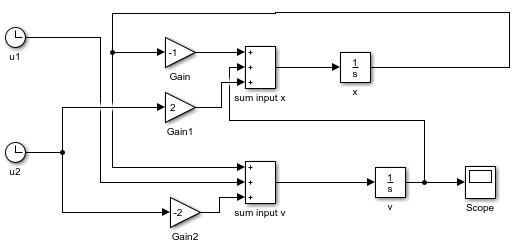
\includegraphics[scale=0.8,angle=90]{\imageDir/aufgabe_b2.JPG}
\caption{Blockschaltbild zum System aus Aufgabe b2}
\label{fig:exercise-b1}
\end{figure}
\newpage

\subsection{Fehlerhaftes System in A, B, C Normalform}
An diesem System ist die $C$-Matrix falsch, da dieses System drei Systemzustände besitzt und daher die $C$-Matrix drei Spalten benötigt, so viele wie es Systemzustände gibt.
\newline
\newline
$
Y=C*X \hspace{5mm} wobei \hspace{3mm} 
X= \begin{bmatrix}
	x \\[0.3em]
	v \\[0.3em]
	z \\[0.3em]
\end{bmatrix}
\hspace{3mm} und \hspace{3mm} 
C = \begin{bmatrix}
	1 & 0 & 0 \\[0.3em]
	2 & 0 & 0 \\[0.3em]
	3 & 0 & 0 \\[0.3em]
\end{bmatrix}
$

\subsection{System als Blockschaltbild und in A, B, C Normalform}
$
X = \begin{bmatrix}
	a \\[0.3em]
	b \\[0.3em]
	c \\[0.3em]
\end{bmatrix}
,
U = \begin{bmatrix}
	i_1 \\[0.3em]
	i_2 \\[0.3em]
\end{bmatrix}
\newline
\newline
\newline
X'=A*X+B*U
\newline
\newline
X'= \begin{bmatrix}
	2 & 4 & -2 \\[0.3em]
	0 & 4 & -1 \\[0.3em]
	0 & 0 & -1 \\[0.3em]
\end{bmatrix}
*
\begin{bmatrix}
	a \\[0.3em]
	b \\[0.3em]
	c \\[0.3em]
\end{bmatrix}
+
\begin{bmatrix}
	2 & 0 \\[0.3em]
	0 & 1 \\[0.3em]
	3 & 0 \\[0.3em]
\end{bmatrix}
*
\begin{bmatrix}
	i_1 \\[0.3em]
	i_2 \\[0.3em]
\end{bmatrix}
\newline
\newline
\newline
\newline
Y=C*X
\newline
\newline
Y=
\begin{bmatrix}
	3 & 0 & 0 \\[0.3em]
	0 & -1 & 0 \\[0.3em]
	1 & 0 & -1 \\[0.3em]
\end{bmatrix}
*
\begin{bmatrix}
	a \\[0.3em]
	b \\[0.3em]
	c \\[0.3em]
\end{bmatrix}
=
\begin{bmatrix}
	(3*a) \\[0.3em]
	(-b) \\[0.3em]
	(a-c) \\[0.3em]
\end{bmatrix}
$

\begin{figure}
\centering
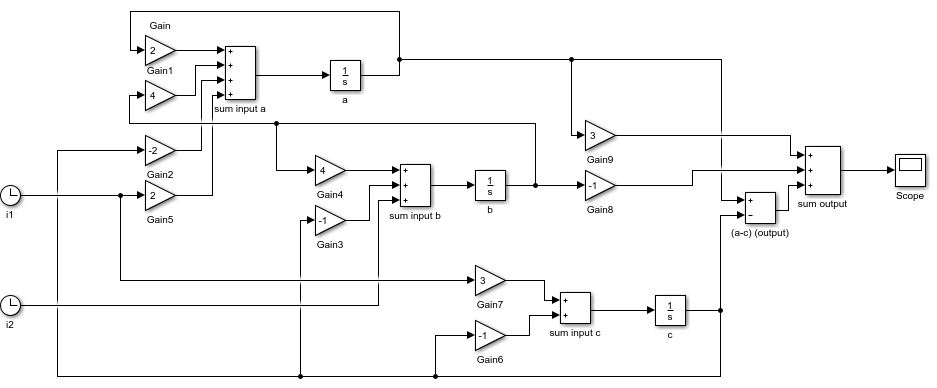
\includegraphics[scale=0.7,angle=90]{\imageDir/aufgabe_b3.JPG}
\caption{Blockschaltbild zum System aus Aufgabe b3}
\label{fig:exercise-b1}
\end{figure}
\ \newpage

\section{Kontinuierliche Simulation}
\label{sec:continous-simulation}
Im Gegensatz zu linearen System können bei nicht linearen Systemen die Werte nicht zu jeden Zeitpunkt berechnet werden. Daher wird bei nicht linearen Systemen die Werteveränderung zum Zeitpunkt $t$ annäherungsweise berechnet. Damit können alle kontinuierlichen Systeme, die durch Differenzialgleichungen dargestellt werden können, simuliert werden. Bei einer richtigen Konfiguration und gewählten Schrittbreite $h$ können die Fehler so klein gehalten werden, dass sie nicht ins Gewicht fallen. 
\newline
\newline
Es ist nicht möglich bei einer annäherungsweisen Berechnungsmethode Fehler vollständig zu vermeiden. Es ist nur möglich den Fehler in einem Bereich zu halten, die für die Simulation akzeptabel ist. Es werden gibt zwei Arten von Fehlern, den lokalen Fehler und den globalen Fehler, wobei der globale Fehler wichtiger ist als der lokale Fehler, der pro Schritt gemacht wird.
\newline
\newline
Aufgrund der annäherungsweisen Berechnung werden Fehler gemacht, die mit den folgend aufgelisteten Methoden minimiert werden können.
\newline
\newline
\textbf{Einschrittmethoden:}
\begin{enumerate}
	\item Euler Integration
	\item Methode von Heun
	\item Runge Kutta
\end{enumerate}
\textbf{Mehrschrittmethoden:}
\begin{enumerate}
	\item Adams Bashford
	\item Adams Moulton
\end{enumerate}
\ \newline
Welche Methode in der Simulation angewendet werden soll, hängt von der Simulation und der akzeptablen Fehlertoleranz der Simulation ab. Meistens wird aber die Methode von \emph{Runge Kutta} als anwendbar angesehen.

\subsection{Euler Integration}
Mit der Euler Integration $y_{i+1}=y_i+h*f(y_i)$, die ein Einschrittverfahren ist, die Änderung über ein Dreieck ermittelt. Dieses Verfahren ist das schnellste der Verfahren, da pro Schritt nur einmal die Funktion $f(y_k)$ aufgerufen werden muss. Der globale Fehler ($O(h)$) verhält sich linear zur gewählten Schrittweite.
\newline
\newline
Bsp.: $h=10 \rightarrow O(h)=10, h=5 \rightarrow O(h)=5$

\begin{figure}[h]
\centering
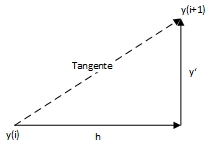
\includegraphics[scale=1]{\imageDir/euler_integration.JPG}
\caption{Dreieck zur Berechnung der Änderung in einem Punkt}
\label{fig:euler-integration}
\end{figure}

\subsection{Methode von Heun}
Mit der Methode von Heun $y_{i+1}=y_i+h/2*(f(y_i) + f(y_i+h*f(y_i)))$, die auch ein Einschrittverfahren ist, wird der nächste Wert im Gegensatz zur Euler Integration über ein Trapez ermittelt. Der globale Fehler ($O(h^2)$) verhält sich quadratisch zur gewählten Schrittbreite $h$. 
\newline
\newline
Bsp.: $h=10 \rightarrow O(h^2)=100, h=5 \rightarrow O(h^2)=25$
\newline
\newline
Der globale Fehler nimmt daher bei geringerer Schrittbreite deutlich mehr ab als bei der Euler Integration.

\begin{figure}[h]
\centering
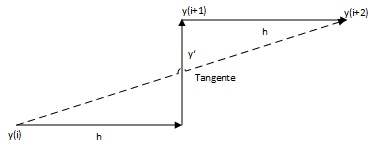
\includegraphics[scale=1]{\imageDir/method_heun.JPG}
\caption{Trapez zur Berechnung der Änderung in einem Punkt}
\label{fig:euler-integration}
\end{figure}

\subsection{Runge Kutta}
Die Methode von Runge Kutta ist ein vierstufiges Einschrittverfahren, das mit Schrittweitenanpassung arbeitet. Es wird ein \emph{Threshold} des erlaubten Fehlers und die neue Schrittweite definiert, die angewendet wird, wenn der \emph{Threshold}  überschritten wird. Mit der dynamischen Anpassung der Schrittweite, kann bei einer Simulation der Rechenaufwand bei wenig Änderungen vermindert werden. Nehmen die Änderungen zu, wird der Fehler bei der Berechnung  größer, wodurch der \emph{Threshold} überschritten wird und Schrittweite auf den eingestellten Wer verkleinert wird. Damit wird der Fehler wieder kleiner, was mit einem verschlechterten Laufzeitverhalten der Simulation einhergeht.

\begin{figure}[h]
\centering
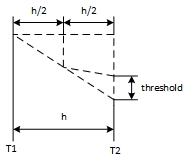
\includegraphics[scale=1]{\imageDir/runge_kutta.JPG}
\caption{Runge Kutta Verfahren mit Schrittweitenanpassung}
\label{fig:euler-integration}
\end{figure}
\ \newpage

\subsection{Mehrstufige Verfahren}
Bei dem Verfahren Adams Bashford werden nur vergangene Werte bei der Berechnung des nächsten Wert miteinbezogen. Bei dem Verfahren Adams Moulton werden zusätzlich zu den vergangen Werten auch angenommene Zukunftswerte bei der Berechnung des nächsten Werts miteinbezogen. Bei beiden Verfahren werden empirische Faktoren verwendet, die sich über die Zeit als gute Faktoren bewährt haben.
\end{document}
